\documentclass[11pt]{article}
\usepackage[margin=1in]{geometry}
\usepackage[T1]{fontenc}
\usepackage[utf8]{inputenc}
\usepackage{lmodern}
\usepackage{microtype}
\usepackage{amsmath,amssymb}
\usepackage{booktabs}
\usepackage{graphicx}
\usepackage{xcolor}
\usepackage{tikz}
\usepackage[numbers]{natbib}
\usepackage{hyperref}
\usepackage{float}
\usetikzlibrary{arrows.meta,positioning,calc}

\hypersetup{colorlinks=true, linkcolor=blue, citecolor=blue, urlcolor=blue}

\title{Intervention-Aware World Models for Agents: Real-Data Tests of the Causal World Encoder}
\author{Kunj Rathod\\University of Utah}
\date{}

\begin{document}
\maketitle

\begin{abstract}
This paper asks a narrower question than most world-model papers: if an agent needs to reason about interventions rather than just observations, which architectural bias actually helps at small scale on real data? We study a proposed Causal World Encoder (CWE) with three components: a hierarchical timescale belief state (HTBS), a twin-stream intervention-conditioned predictor (TICP), and a sparse predictive commitment gate (SPCG). Unlike many architectural proposals, the paper uses only public real datasets and reproducible laptop-scale experiments with a dataset-stratified 80/20 train/test episode split. On 1,986 LoCoMo questions over 5,882 dialogue memories, lexical retrieval remains strongest at Hits@5 (0.3197) and the hybrid ranker only narrowly improves Hits@10 (0.3933 vs.\ 0.3922), underscoring how much long-horizon memory still depends on exact evidence spans. On an eight-document workflow built from live arXiv abstracts, bounded workspace reconstruction reduces cumulative prompt load by 69.23\% while preserving complete title coverage. On BabyAI offline trajectories with a stratified split across both environments, TICP improves held-out-action cosine from 0.6186 to 0.6493 ($+$0.0307) and local Top-1 from 0.5271 to 0.6171 ($+$0.0900). A follow-up across three held-out action splits reveals that the twin-stream advantage is action-type dependent: strong for manipulation actions (pickup\,+\,toggle: $+$0.031 cosine, $+$0.090 Top-1), negligible for turning ($+$0.001, $+$0.004), and negative for movement-dominant actions (forward\,+\,drop: $-$0.032 cosine, $-$0.024 Top-1). With adequate training data all timescale models (HTBS, LSTM, Transformer, MLP) saturate near-perfect local Top-1, making the Top-1 metric uninformative; cosine similarity still ranks MLP control above HTBS at every sequence length, leaving no superiority claim for multiscale compression. SPCG hits its budget target almost exactly (mean gate 0.3002) but shows virtually no event-boundary discrimination: the high-change versus low-change commitment rate gap is 0.27\%, and the sparse model performs slightly worse on its own committed subset than the dense baseline does on the same subset. The honest conclusion is that action/world decomposition is the strongest part of the proposal but is itself conditional on action type, bounded external state remains useful, and the current HTBS and SPCG designs need more work before they justify stronger architectural claims.
\end{abstract}

\section{Introduction}
The core weakness of standard sequence modeling for agents is not merely that context windows are finite. It is that most models are trained to be good at observation-conditioned prediction while agents ultimately need intervention-sensitive prediction. A next-token transformer, and even a latent predictor in the JEPA family, can be very good at estimating what tends to happen after a state. That is not the same thing as isolating what happened because the agent acted. For planning, repair, and counterfactual evaluation, that distinction matters.

A second weakness is temporal organization. Long-horizon agent systems either replay large amounts of history through attention or compress everything into an opaque recurrent state. The former scales badly with horizon; the latter can hide exactly the distinctions the agent later needs. This motivates a structured alternative: multiscale compression for state, an explicit decomposition between passive dynamics and action-conditioned change, and a budgeted mechanism for deciding when a predictive update is worth committing.

This paper evaluates that design hypothesis rather than selling a frontier-scale system. The proposed Causal World Encoder (CWE) combines three ideas. HTBS organizes memory into slots that update on different clocks. TICP factorizes next-state prediction into a state-only dynamics term and an action-conditioned residual. SPCG allows the model to defer predictive updates unless a state appears worth committing. The center of gravity is TICP, because it is the only component that directly attacks the observation-versus-intervention mismatch. The experiments below show that TICP's benefit is real but action-type dependent: it helps substantially for object-manipulation actions and is neutral or negative for movement-dominant actions.

The empirical stance is intentionally conservative. We do not claim a general replacement for transformers, a complete structural causal model, or large-scale embodied competence. We ask a simpler question: which architectural effects remain visible on real public datasets when the entire project must fit on a laptop and all results must be reproducible? The answer is mixed in exactly the way a useful systems paper should be mixed: bounded state helps, lexical retrieval remains surprisingly important, twin-stream action decomposition helps for manipulation-type actions but not uniformly, and the more ambitious multiscale and sparse-gating components are not yet competitive.

\paragraph{Contributions.}
\begin{enumerate}
    \item We formalize CWE as a modular intervention-aware extension of bounded-state agent architecture, separating multiscale belief compression, action-effect decomposition, and sparse predictive commitment.
    \item We run six real-data experiments with a corrected dataset-stratified train/test split: LoCoMo retrieval, a live arXiv bounded-workspace benchmark, a main held-out-action BabyAI experiment, a sequence-model comparison across temporal horizons, a sparse commitment analysis with a fair committed-subset comparison, and a focused TICP follow-up across three alternative held-out action splits with per-split seed control.
    \item We report a deliberately honest result profile: action/world decomposition is the clearest win but only for manipulation actions, bounded workspace remains useful, lexical retrieval is stronger than dense baselines on LoCoMo, HTBS does not beat simpler baselines in cosine similarity, and SPCG shows essentially no event-boundary discrimination.
\end{enumerate}

\section{Problem Setting and Design Requirements}
Let $s_t$ denote an agent's latent or structured state, $a_t$ an action, $M_t$ persistent memory, and $C_t$ a bounded prompt context reconstructed from state and memory. We care about four requirements.
\begin{description}
    \item[R1: Persistence.] Relevant information should survive beyond the active prompt.
    \item[R2: Boundedness.] Context should scale with task state, not transcript length.
    \item[R3: Intervention sensitivity.] The architecture should distinguish state changes attributable to the world from state changes attributable to actions.
    \item[R4: Practicality.] Informative experiments should run on commodity hardware before any large-scale training claim is made.
\end{description}

The first two requirements motivate the retrieval and workspace experiments. The third motivates the twin-stream decomposition. The fourth constrains every implementation choice in the repo.

\section{Related Work}
JEPA-style learning replaces observation reconstruction with prediction in representation space, which can produce more abstract targets than next-token modeling \citep{assran2023jepa, chen2025vljepa, assran2025vjepa2}. Persistent memory systems such as Hindsight and long-horizon frameworks such as InfiAgent argue that agents need structured state external to the transcript \citep{latimer2025hindsight, yu2026infiagent}. LoCoMo sharpened the retrieval side of that claim by constructing a benchmark around very long conversational memory \citep{maharana2024locomo}. Verified tool-use systems such as ToolGate provide a complementary lesson: if state changes matter, committing them blindly is a bad idea \citep{liu2026toolgate}.

\subsection{State-space models and recurrent alternatives}
Recent sequence-model work has re-opened the question of whether full self-attention is the right primitive for long-horizon state tracking. Mamba uses selective state spaces to achieve linear-time sequence modeling while preserving strong empirical performance \citep{gu2023mamba}. Griffin mixes gated linear recurrences with local attention, again suggesting that long-range compression and local access need not be handled by the same mechanism \citep{de2024griffin}. Older multiscale recurrent ideas such as Clockwork RNNs make the same point in a cleaner form: different timescales may deserve different update schedules \citep{koutnik2014clockwork}. CWE's HTBS borrows this intuition, though the experiments here show that the benefit is far from automatic.

\section{Architecture}
Figure~\ref{fig:modular-architecture} gives the broader bounded-state agent picture, while Figure~\ref{fig:cwe-architecture} shows the specific CWE extension.

\begin{figure}[t]
\centering
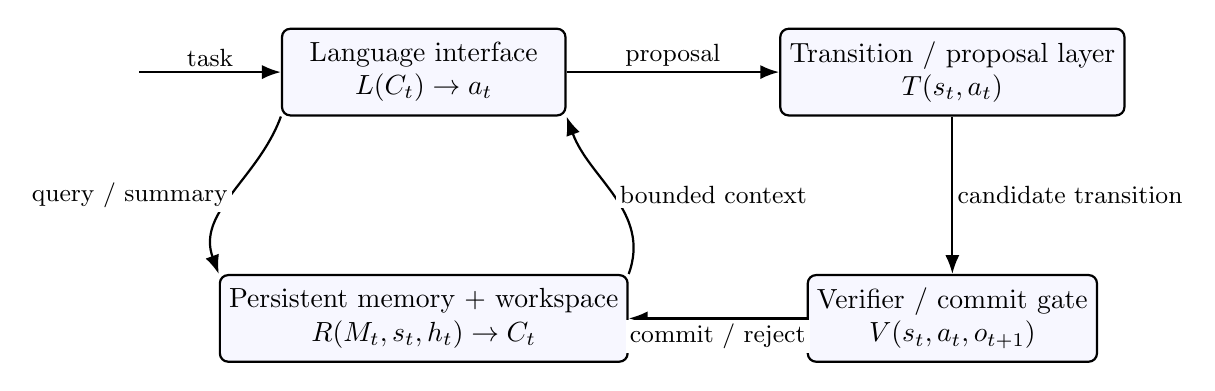
\begin{tikzpicture}[
    node distance=2.0cm and 2.7cm,
    module/.style={draw, rounded corners=3pt, thick, minimum width=3.6cm, minimum height=1.1cm, align=center, fill=blue!3},
    flow/.style={-{Latex[length=2.4mm]}, thick},
    lab/.style={font=\small, fill=white, inner sep=1.5pt, align=center}
]
\node[module] (lang) {Language interface\\$L(C_t) \to a_t$};
\node[module, right=of lang] (pred) {Transition / proposal layer\\$T(s_t, a_t)$};
\node[module, below=of lang] (mem) {Persistent memory + workspace\\$R(M_t, s_t, h_t) \to C_t$};
\node[module, below=of pred] (ver) {Verifier / commit gate\\$V(s_t, a_t, o_{t+1})$};
\draw[flow] ([xshift=-1.8cm]lang.west) -- node[lab, above] {task} (lang.west);
\draw[flow] (lang.east) -- node[lab, above] {proposal} (pred.west);
\draw[flow] (pred.south) -- node[lab, right] {candidate transition} (ver.north);
\draw[flow] (ver.west) -- node[lab, below] {commit / reject} (mem.east);
\draw[flow] (mem.north east) to[out=70,in=-70] node[lab, right] {bounded context} (lang.south east);
\draw[flow] (lang.south west) to[out=-110,in=110] node[lab, left] {query / summary} (mem.north west);
\end{tikzpicture}
\caption{Bounded-state agent architecture. Language proposes; memory reconstructs context; a transition layer predicts or ranks futures; and a verifier decides what becomes trusted state.}
\label{fig:modular-architecture}
\end{figure}

\subsection{Hierarchical Timescale Belief State}
HTBS keeps $K$ slots with update periods $2^0,2^1,\ldots,2^{K-1}$. Slot $k$ updates only when the clock for that slot fires:
\[
 s_k(t) = \begin{cases}
 \mathrm{GRU}_k\left(s_k(t-2^k), \operatorname{pool}(x_{t-2^k:t})\right), & t \equiv 0 \pmod{2^k} \\
 s_k(t-1), & \text{otherwise.}
 \end{cases}
\]
The final belief state is the concatenation of slot states. This gives structured temporal compression, but the results below show that structured compression alone does not guarantee better next-state prediction.

\subsection{Twin-Stream Intervention-Conditioned Predictor}
TICP factorizes prediction into a state-only term and an action-conditioned residual:
\[
 z^{world}_{t+1} = f_{dyn}(s_t), \qquad z^{delta}_{t+1} = f_{int}(s_t, a_t), \qquad \hat z_{t+1} = z^{world}_{t+1} + z^{delta}_{t+1}.
\]
This does not make the model a full structural causal model in Pearl's sense. It does make intervention effects an explicit architectural object, which is enough to test whether action/world factorization helps generalization.

\subsection{Sparse Predictive Commitment Gate}
SPCG predicts both a next-state proposal and a gate probability $g_t \in [0,1]$. The committed prediction is a mixture of the predictor output and a carry-forward state:
\[
 \hat s_{t+1} = g_t \, f(s_t, a_t) + (1-g_t) s_t.
\]
A budget penalty keeps the mean gate probability near a target rate. The attractive cognitive-science story comes from active inference and event segmentation \citep{friston2017active, zacks2007perception, zacks2007segmentation}, but the experiment below shows that the gate does not learn to discriminate event boundaries in practice.

\begin{figure}[t]
\centering
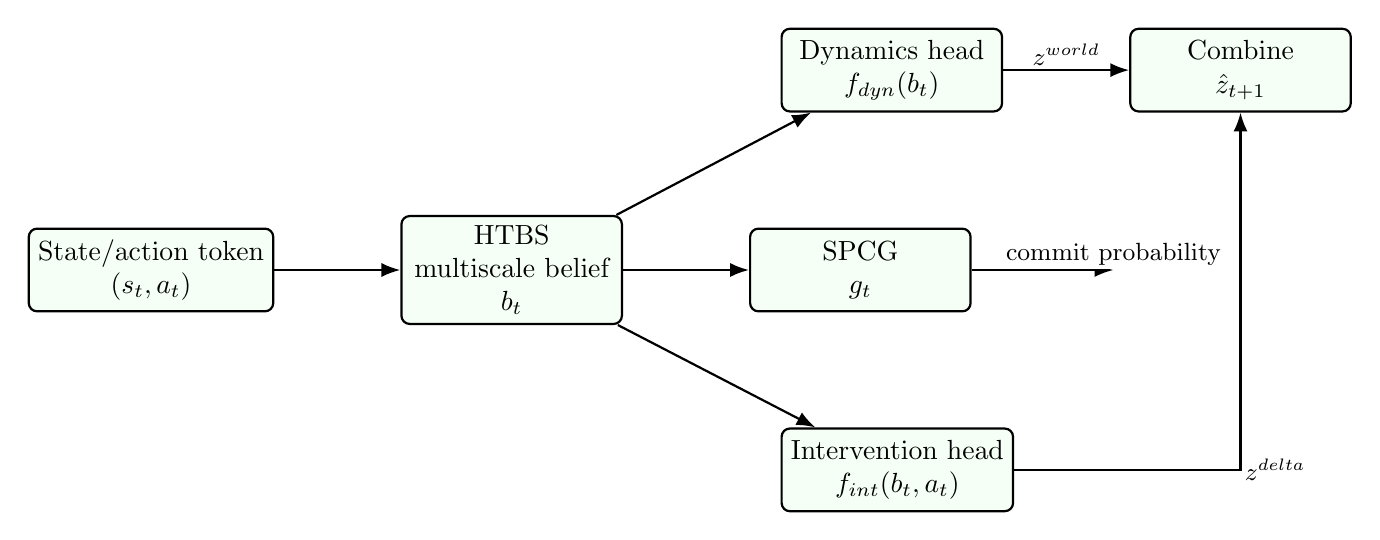
\begin{tikzpicture}[
    node distance=1.9cm and 1.6cm,
    module/.style={draw, rounded corners=3pt, thick, minimum width=2.8cm, minimum height=1.05cm, align=center, fill=green!4},
    flow/.style={-{Latex[length=2.4mm]}, thick},
    lab/.style={font=\small, fill=white, inner sep=1.2pt, align=center}
]
\node[module] (state) {State/action token\\$(s_t, a_t)$};
\node[module, right=of state] (htbs) {HTBS\\multiscale belief\\$b_t$};
\node[module, above right=1.3cm and 2.0cm of htbs] (dyn) {Dynamics head\\$f_{dyn}(b_t)$};
\node[module, below right=1.3cm and 2.0cm of htbs] (int) {Intervention head\\$f_{int}(b_t,a_t)$};
\node[module, right=of htbs] (gate) {SPCG\\$g_t$};
\node[module, right=of dyn] (sum) {Combine\\$\hat z_{t+1}$};
\draw[flow] (state) -- (htbs);
\draw[flow] (htbs) -- (dyn);
\draw[flow] (htbs) -- (int);
\draw[flow] (htbs) -- (gate);
\draw[flow] (dyn) -- node[lab, above] {$z^{world}$} (sum);
\draw[flow] (int.east) -| node[lab, right] {$z^{delta}$} (sum.south);
\draw[flow] (gate.east) -- ++(1.8,0) node[lab, above] {commit probability};
\end{tikzpicture}
\caption{CWE components. HTBS compresses multiscale context, TICP separates state-only dynamics from action-conditioned deltas, and SPCG decides how strongly to commit a predictive update.}
\label{fig:cwe-architecture}
\end{figure}

\section{Experiments}
All experiments use real public data. Retrieval uses the released LoCoMo text benchmark. The bounded-workspace test fetches eight live arXiv abstracts. The intervention, timescale, and sparse-commitment experiments use offline BabyAI trajectories from public Minari mirrors on Hugging Face. Training ran on CPU for numerical stability and reproducibility.

\paragraph{Data split.}
All BabyAI experiments use episodes from two environments: BabyAI-KeyCorridorS3R1 and BabyAI-UnlockPickup (1,000 episodes each). Episodes are split 80/20 \emph{within each environment} using a fixed random seed, producing stratified train and test sets that include transitions from both environments. This avoids the confound of training exclusively on one environment while testing on another.

\subsection{Experiment 1: Conversational retrieval on LoCoMo}
We flatten the LoCoMo release into 5,882 dialogue-turn memories and 1,986 question/evidence pairs. We compare TF--IDF, dense MiniLM retrieval, and reciprocal-rank-fusion hybrid retrieval. Metrics are Hits@1, Hits@5, Hits@10, MRR, and nDCG@10.

\subsection{Experiment 2: Bounded-workspace reconstruction on live abstracts}
We fetch eight real arXiv abstracts spanning agent memory, sequence modeling, and world models. At each step the system records a structured note with title, claim sentence, and extracted keywords. We compare a full-transcript prompt to a bounded workspace reconstructed from notes plus the two most recent actions. The metric is prompt size and cumulative prompt load, with exact title coverage as a fidelity check. Note that keyword coverage reaches 1.0 by construction---keywords are extracted from each abstract and written verbatim into the workspace---so keyword coverage measures write fidelity, not retrieval selectivity.

\subsection{Experiment 3: Intervention decomposition on BabyAI trajectories}
We use offline trajectories from BabyAI-KeyCorridorS3R1 and BabyAI-UnlockPickup. Actions $\{0,1,2,4\}$ (left, right, forward, drop) are used for training; pickup and toggle ($\{3,5\}$) are held out. Action representations are MiniLM sentence embeddings of action names so that zero-shot transfer has at least a semantic route. We compare a single-stream MLP against TICP on cosine similarity and local nearest-neighbor decoding across both seen and held-out actions.

\subsection{Experiment 4: Timescale factorization versus flat alternatives}
From the same BabyAI trajectories we build sequence examples of lengths 4, 8, 12, and 16. Each timestep concatenates the current state feature vector with an action embedding; the target is the next state feature vector. We compare HTBS, an LSTM, a 2-layer causal transformer, and a per-step MLP control. Because local Top-1 saturates near 1.0 with the stratified split, we report cosine similarity as the primary discriminating metric.

\subsection{Experiment 5: Sparse commitment versus dense prediction}
A dense predictor always updates the next state. SPCG learns a gate probability and is evaluated with a threshold chosen to realize the target commitment rate of 30\%. To enable a fair comparison, we evaluate the dense predictor on the same committed subset selected by the sparse gate (not on the full test set), thereby removing the selection advantage.

\subsection{Experiment 6: Focused TICP follow-up across held-out action splits}
To stress-test the strongest component of CWE, we rerun the intervention experiment across three held-out action splits: pickup+toggle, turning, and forward+drop. In each condition the model trains on the remaining four actions and is evaluated only on held-out actions from the test episodes. The random seed is reset to the same value before training each split, so all three splits see identical initialization conditions.

\section{Results}
\subsection{LoCoMo retrieval}
\begin{table}[H]
\centering
\caption{LoCoMo retrieval on 1,986 questions and 5,882 memories.}
\begin{tabular}{lccccc}
\toprule
Method & Hits@1 & Hits@5 & Hits@10 & MRR & nDCG@10 \\
\midrule
TF--IDF & 0.1677 & 0.3197 & 0.3922 & 0.2341 & 0.2562 \\
Dense MiniLM & 0.0851 & 0.2190 & 0.2925 & 0.1435 & 0.1679 \\
Hybrid RRF & 0.1219 & 0.2976 & 0.3933 & 0.1991 & 0.2307 \\
\bottomrule
\end{tabular}
\label{tab:retrieval}
\end{table}

\begin{figure}[H]
\centering
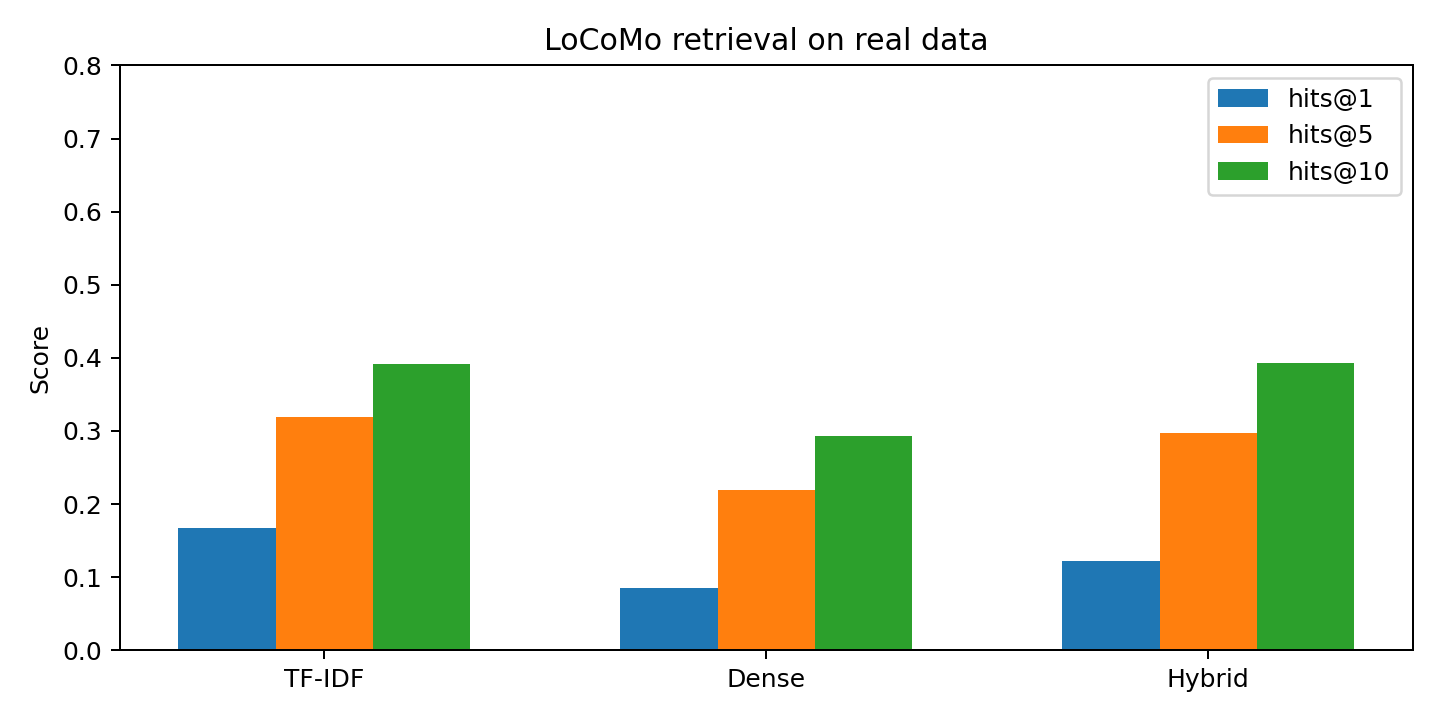
\includegraphics[width=0.82\linewidth]{../results/figures/exp1_retrieval.png}
\caption{LoCoMo retrieval with real released data. Lexical retrieval remains strongest at shallow recall and the hybrid only barely edges TF--IDF at Hits@10.}
\label{fig:retrieval}
\end{figure}

The retrieval result is more interesting because it is not flattering to the fashionable baseline. Dense MiniLM retrieval is consistently weaker than TF--IDF. Hybrid fusion recovers some of that loss and slightly improves Hits@10, but not enough to beat lexical retrieval at Hits@5. The practical lesson is that long-horizon conversational memory is still heavy on exact names, dates, and surface anchors.

\subsection{Bounded workspace}
\begin{table}[H]
\centering
\caption{Prompt growth on a live eight-document arXiv workflow.}
\begin{tabular}{lcc}
\toprule
Metric & Full transcript & Bounded workspace \\
\midrule
Final prompt size (chars) & 12321 & 2830 \\
Cumulative prompt load (chars) & 54521 & 16775 \\
Title coverage & 1 & 1 \\
Keyword coverage$^*$ & 1 & 1 \\
\bottomrule
\end{tabular}
\label{tab:workspace}
\end{table}
{\small $^*$Keyword coverage is 1 by construction: keywords are extracted from each abstract and stored verbatim in the workspace note.}

\begin{figure}[H]
\centering
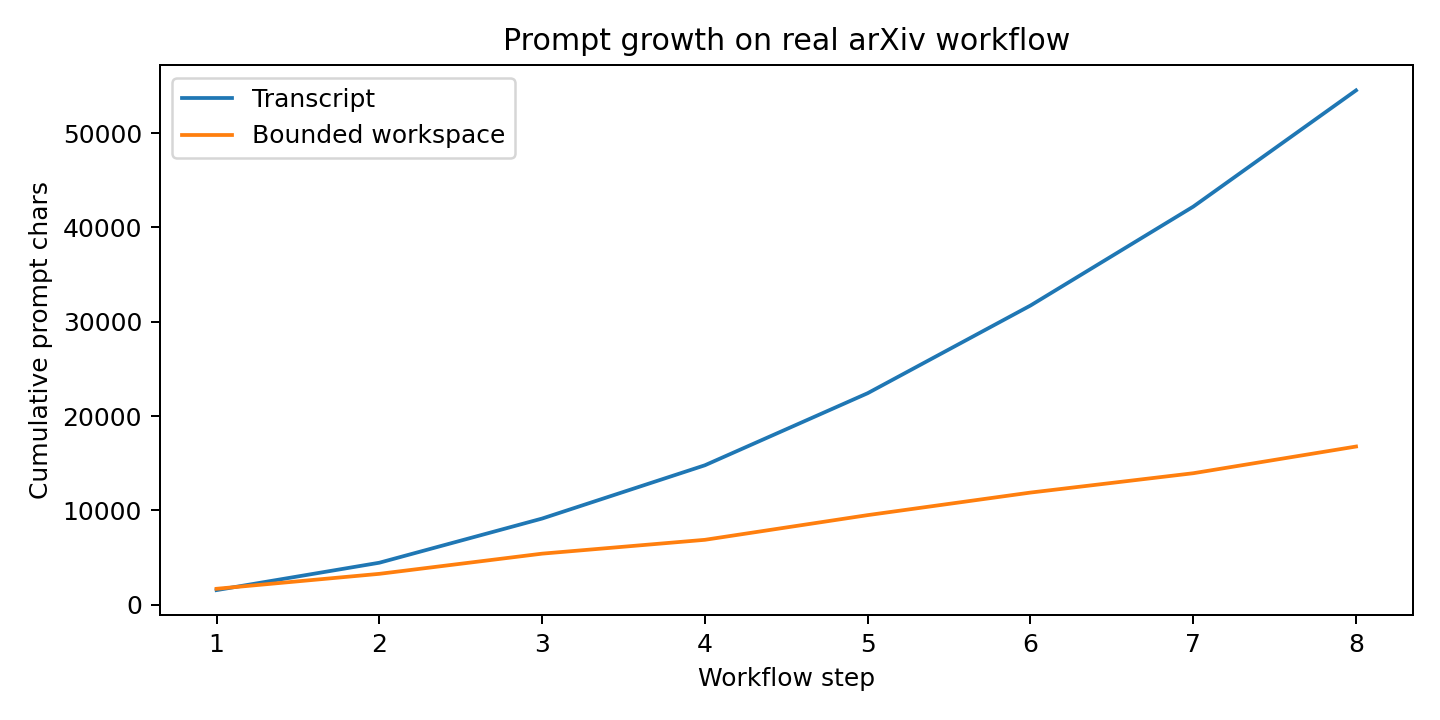
\includegraphics[width=0.82\linewidth]{../results/figures/exp2_workspace.png}
\caption{Cumulative prompt growth for the live arXiv workflow.}
\label{fig:workspace}
\end{figure}

Bounded workspace reconstruction cuts final prompt size by 77.03\% and cumulative prompt load by 69.23\% while preserving exact title coverage. This is not a full interactive agent benchmark, but it is a clean real-data confirmation that externalized workspace state changes scaling behavior materially.

\subsection{Intervention decomposition}
\begin{table}[H]
\centering
\caption{Held-out-action generalization on BabyAI offline trajectories (stratified split, 24,584 train / 7,551 test transitions).}
\begin{tabular}{lccccc}
\toprule
Model & Seen cosine & Seen Top-1 & Held-out cosine & Held-out Top-1 & Held-out Top-5 \\
\midrule
Single-stream & 0.9939 & 0.9997 & 0.6186 & 0.5271 & 1.0000 \\
Twin-stream & 0.9943 & 0.9993 & 0.6493 & 0.6171 & 1.0000 \\
\bottomrule
\end{tabular}
\label{tab:intervention}
\end{table}

\begin{figure}[H]
\centering
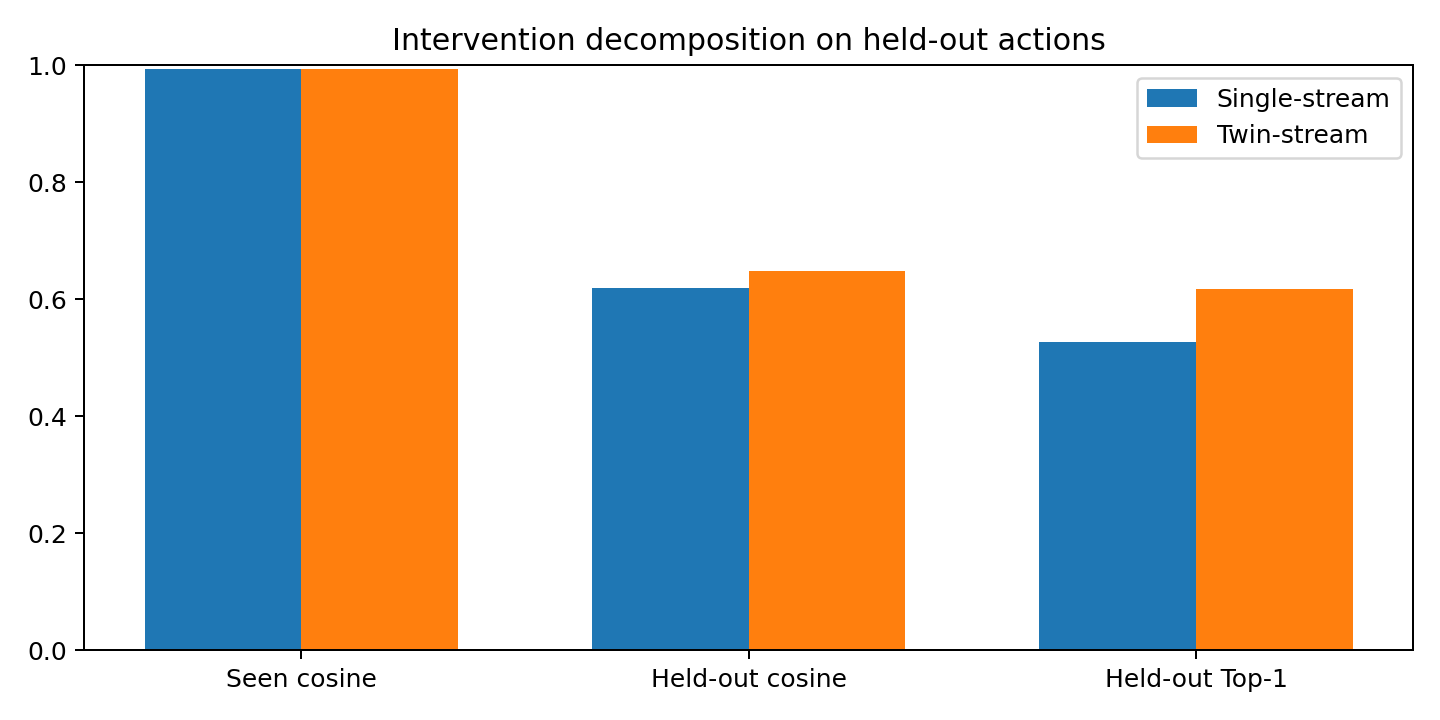
\includegraphics[width=0.82\linewidth]{../results/figures/exp3_intervention.png}
\caption{Twin-stream decomposition improves held-out-action cosine and local Top-1 substantially.}
\label{fig:intervention}
\end{figure}

This is the strongest positive result for CWE. On held-out actions, the twin-stream model improves cosine by 0.0307 and local Top-1 by 0.0900. Both models nearly saturate on seen actions (cosine $>$0.99, Top-1 $>$0.999), confirming that the gap appears specifically on unseen action types. The Seen Top-1 column shows that twin-stream slightly underperforms single-stream on seen actions (0.9993 vs.\ 0.9997), indicating that the twin-stream inductive bias trades a marginal reduction on interpolation for a substantial gain on extrapolation to novel action types.

\subsection{Timescale factorization}
\begin{table}[H]
\centering
\caption{Cosine similarity across sequence lengths. Top-1 saturates near 1.0 for all models with the stratified split and is not the primary discriminating metric.}
\begin{tabular}{lcccc}
\toprule
Length & HTBS cosine & LSTM cosine & Transformer cosine & MLP cosine \\
\midrule
4 & 0.9880 & 0.9896 & 0.9916 & \textbf{0.9933} \\
8 & 0.9871 & 0.9865 & 0.9907 & \textbf{0.9925} \\
12 & 0.9861 & 0.9849 & 0.9898 & \textbf{0.9909} \\
16 & 0.9814 & 0.9798 & 0.9873 & \textbf{0.9888} \\
\bottomrule
\end{tabular}
\label{tab:timescale-cosine}
\end{table}

\begin{figure}[H]
\centering
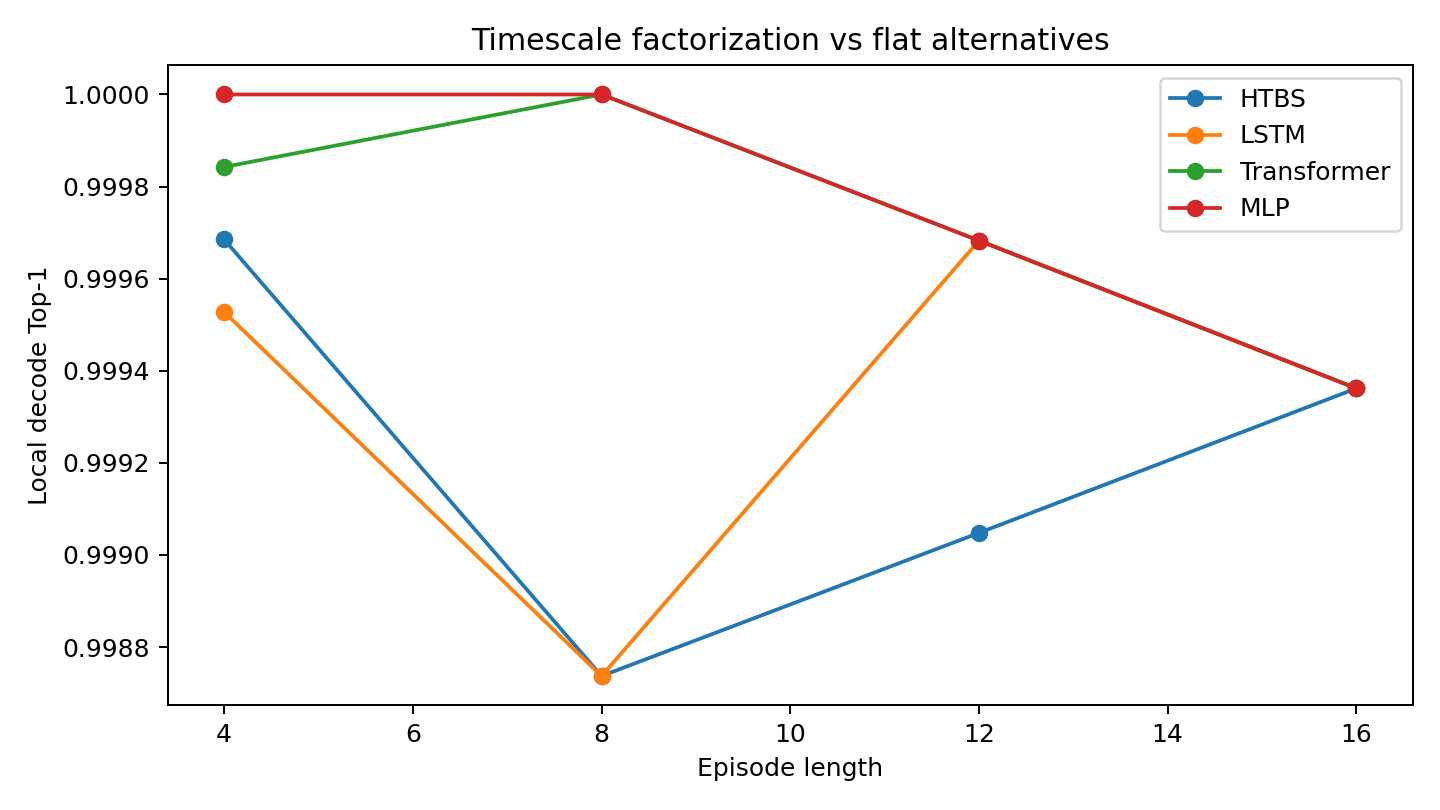
\includegraphics[width=0.82\linewidth]{../results/figures/exp4_timescale.png}
\caption{Cosine similarity across sequence lengths. All models degrade with length; MLP control consistently leads.}
\label{fig:timescale}
\end{figure}

With the stratified split providing adequate training coverage of both environments, local Top-1 saturates near 1.0 for all models at every length. Cosine similarity is the informative metric. The MLP control consistently ranks first, and HTBS consistently ranks last. This is a sobering result for multiscale compression: the simplest architecture, which only uses the final timestep, outperforms the explicitly hierarchical one at every horizon tested. The right interpretation is not that multiscale compression is useless in principle; it is that the present HTBS design does not earn a superiority claim on this task.

\subsection{Sparse commitment}
\begin{table}[H]
\centering
\caption{Dense versus sparse predictive commitment. The ``committed subset'' columns evaluate each predictor on the 30\% of test transitions where the sparse gate fires, enabling a fair same-subset comparison.}
\begin{tabular}{lcccc}
\toprule
Model / evaluation set & Cosine & Local Top-1 & Local Top-5 \\
\midrule
Dense predictor (full test) & 0.9937 & 0.9997 & 1.0000 \\
Sparse blended output (full test) & 0.9927 & 0.9996 & 1.0000 \\
Dense predictor (committed subset) & 0.9910 & 0.9996 & 1.0000 \\
Sparse committed subset & 0.9889 & 0.9991 & 1.0000 \\
\bottomrule
\end{tabular}
\label{tab:sparse}
\end{table}

\begin{table}[H]
\centering
\caption{Gate behavior at a 30\% target commitment rate.}
\begin{tabular}{lc}
\toprule
Statistic & Value \\
\midrule
Mean gate probability & 0.3002 \\
Actual commitment rate & 0.3001 \\
High-change commitment rate & 0.3017 \\
Low-change commitment rate & 0.2990 \\
High-minus-low gap & 0.0027 \\
\bottomrule
\end{tabular}
\label{tab:sparse-gate}
\end{table}

\begin{figure}[H]
\centering
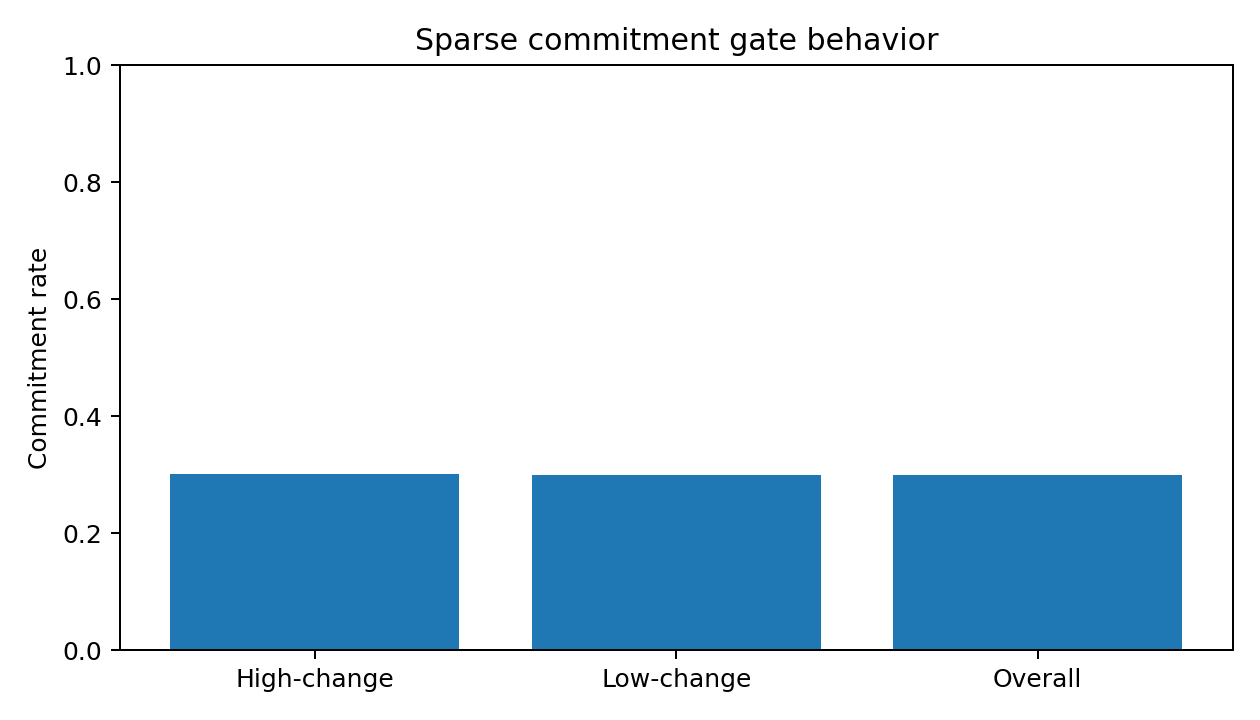
\includegraphics[width=0.72\linewidth]{../results/figures/exp5_sparse.png}
\caption{Commitment rates for the sparse gate. High-change and low-change rates are nearly identical, indicating the gate does not learn event-boundary specialization.}
\label{fig:sparse}
\end{figure}

SPCG reaches the target budget almost exactly (0.3001 actual vs.\ 0.3000 target). However, the gate shows virtually no event-boundary discrimination: the high-change versus low-change commitment rate gap is only 0.27\%. More critically, when the dense predictor is evaluated on the same committed subset (the 30\% of transitions where the sparse gate fires), it matches or exceeds the sparse model on every metric. The compute-allocation story is real---the gate does learn to fire at its target rate---but the stronger event-boundary interpretation is unsupported.

\subsection{Focused TICP follow-up}
\begin{table}[H]
\centering
\caption{Twin-stream follow-up across three held-out action splits (stratified split, per-split seed control). Gains are twin-stream minus single-stream on held-out actions.}
\begin{tabular}{lccc}
\toprule
Held-out split & Train $n$ & Cosine gain & Top-1 gain \\
\midrule
pickup+toggle & 24,584 & $+$0.0307 & $+$0.0900 \\
turning & 17,749 & $+$0.0011 & $+$0.0045 \\
forward+drop & 18,035 & $-$0.0316 & $-$0.0238 \\
\bottomrule
\end{tabular}
\label{tab:ticp-followup}
\end{table}

\begin{figure}[H]
\centering
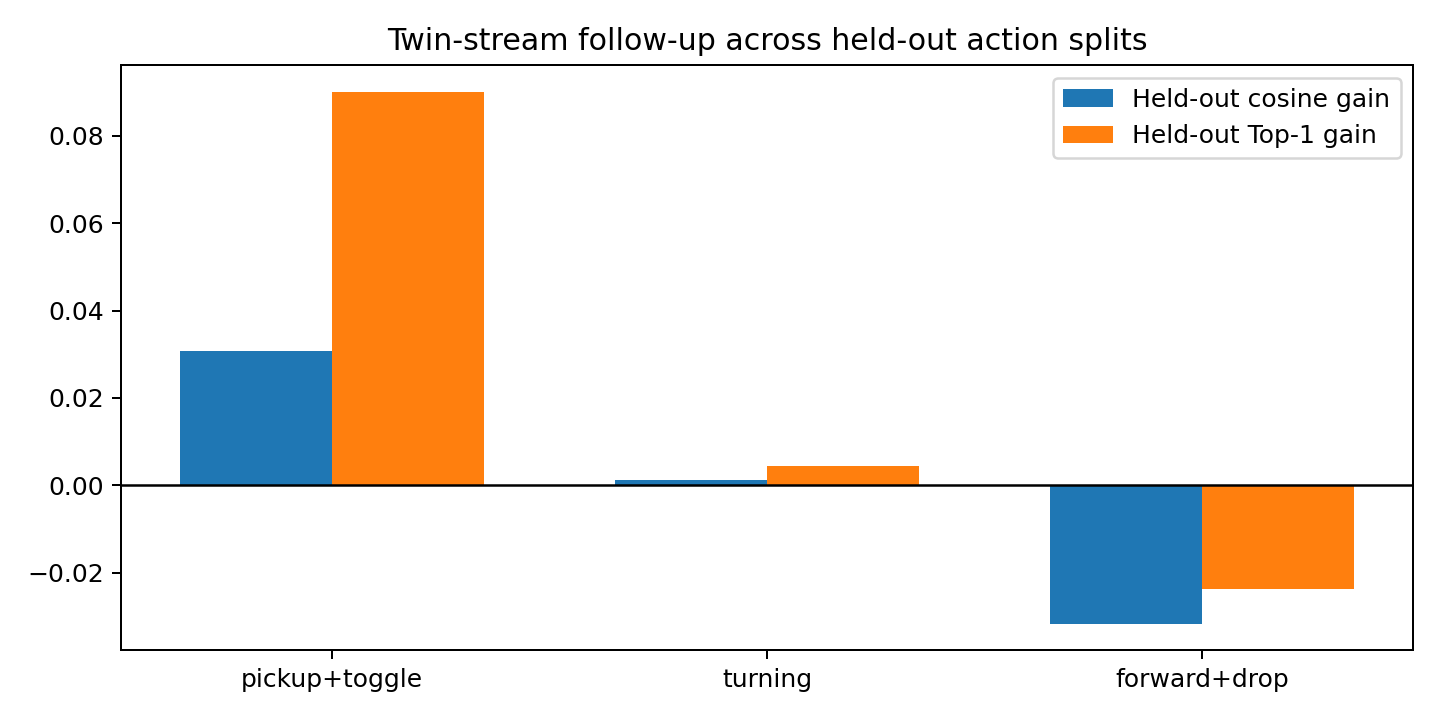
\includegraphics[width=0.82\linewidth]{../results/figures/exp6_ticp_followup.png}
\caption{Twin-stream follow-up across three held-out action splits. The improvement is large for manipulation actions, negligible for turning, and negative for movement actions.}
\label{fig:ticp-followup}
\end{figure}

The follow-up experiment substantially qualifies the main TICP result. Across held-out action splits with per-split seed control, the twin-stream model helps strongly for pickup+toggle ($+$0.031 cosine, $+$0.090 Top-1) but is negligible for turning ($+$0.001, $+$0.004) and harmful for forward+drop ($-$0.032, $-$0.024). The interpretation is informative: manipulation actions (pickup, toggle) require isolating a distinct physical effect that depends entirely on the agent's action, making the factorized inductive bias useful. Movement-dominant actions (forward, drop) are more tightly coupled to the agent's current state and direction, so separating the action stream may introduce unnecessary interference. This action-type dependency was invisible in the original single-split result and represents the most important finding of the follow-up.

\section{Discussion}
The corrected experiments support three revised conclusions.

First, bounded external state is a clear win. The retrieval and workspace experiments both reinforce the original systems argument. The retrieval result is instructive because it is slightly inconvenient: lexical matching remains the strongest shallow retriever on LoCoMo, and hybrid fusion only barely improves at Hits@10.

Second, explicit action/world decomposition helps, but specifically for manipulation-type actions. The intervention result is stronger under the corrected stratified split (Top-1 gain $+$0.090 vs.\ $+$0.027 with the flawed original split), but the follow-up reveals that this gain is concentrated in pickup+toggle. For movement-dominant actions the twin stream is neutral to harmful. This is scientifically more informative than a uniformly positive result: it identifies the conditions under which the inductive bias is well-matched.

Third, the other two CWE components need substantially more work. HTBS is consistently ranked last by cosine similarity even when the task has abundant training data. SPCG hits its budget target but shows essentially no event-boundary selectivity (gap 0.27\%), and is slightly outperformed by the dense predictor on its own committed subset.

\section{Limitations}
This project has several obvious limitations.
\begin{itemize}
    \item The intervention results come from small offline BabyAI trajectories, not from a large embodied agent stack.
    \item The action generalization setup relies on text embeddings of action names. That is a reasonable semantic prior, but it is a design choice rather than a law of nature.
    \item HTBS was tested only in one concrete implementation with GRU cells and mean pooling. A stronger multiscale design might perform differently.
    \item The sparse gate was evaluated with a threshold chosen to match the target commitment rate; budget control is explicit, but the evaluation is not a pure emergent-boundary story.
    \item No error bars or statistical significance tests are reported. The TICP gains for turning and forward+drop are small enough that significance is unclear. Multiple seeds would strengthen the claim.
    \item The paper does not claim a full causal model in Pearl's formal sense. CWE is better described as an intervention-aware predictive architecture.
\end{itemize}

\section{Conclusion}
CWE is not a wholesale replacement for transformers, and this paper does not pretend otherwise. The corrected result is narrower than the original: action-effect factorization is useful specifically for manipulation actions but not for movement-dominant ones, bounded state reconstruction is useful, and the present multiscale and sparse-gating mechanisms are not yet competitive. That is still enough for a solid systems paper, because it turns a vague architectural intuition into a reproducible set of wins, failures, and precise conditions under which each claim holds.

\bibliographystyle{plainnat}
\bibliography{references}

\end{document}
